\documentclass[tikz,border=6pt]{standalone}
\usepackage{tikz}
\usepackage{amsmath,amssymb,bm}
\usetikzlibrary{shapes.geometric, arrows.meta, positioning, fit,
                backgrounds, calc}

\definecolor{choice}{RGB}{240,210,60}
\definecolor{outcome}{RGB}{70,130,180}
\definecolor{markov}{RGB}{31,119,180}
\definecolor{renew}{RGB}{44,160,44}

\begin{document}
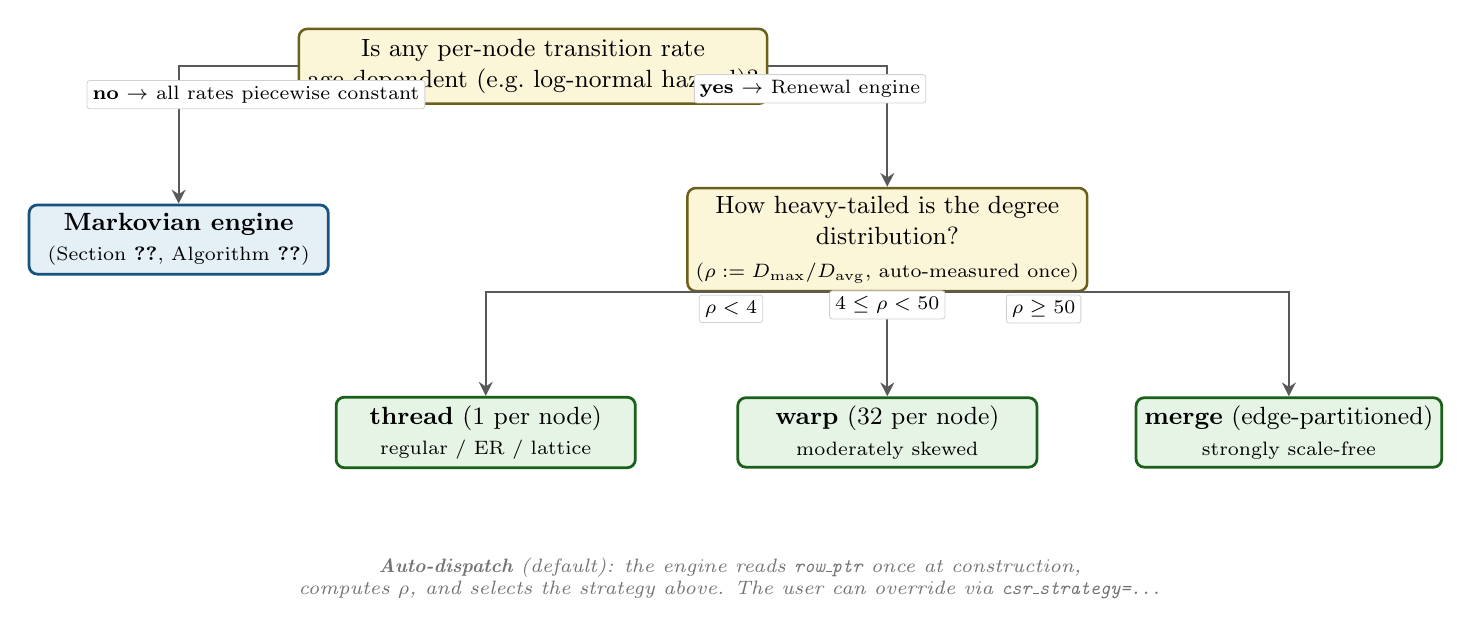
\begin{tikzpicture}[
    question/.style={rectangle, rounded corners=3pt,
                     draw=choice!45!black, line width=0.9pt,
                     fill=choice!20, align=center, font=\small,
                     minimum width=4.7cm, minimum height=0.95cm,
                     inner sep=3pt},
    outcomeA/.style={rectangle, rounded corners=3pt,
                     draw=markov!70!black, line width=1pt,
                     fill=markov!12, align=center, font=\small,
                     minimum width=3.8cm, minimum height=0.85cm,
                     inner sep=3pt},
    outcomeB/.style={rectangle, rounded corners=3pt,
                     draw=renew!60!black, line width=1pt,
                     fill=renew!12, align=center, font=\small,
                     minimum width=3.8cm, minimum height=0.85cm,
                     inner sep=3pt},
    thresh/.style={rectangle, fill=white, inner sep=2pt,
                   rounded corners=1pt, draw=black!18,
                   font=\scriptsize, line width=0.3pt},
    flow/.style={-{Stealth[length=5pt,width=5pt]}, line width=0.8pt,
                 color=black!65},
]

% ==========================================================
% Top-level question: is the model age-dependent?
% ==========================================================
\node[question] (q1) at (0, 4.2)
    {Is any per-node transition rate\\ age-dependent
     (e.g.\ log-normal hazard)?};

% -------- NO branch: Markovian engine -----------
\node[outcomeA] (markov) at (-4.5, 2.0)
    {\textbf{Markovian engine}\\
     \scriptsize(Section~\ref{sec:markov_engine}, Algorithm~\ref{alg:markov})};
\draw[flow] (q1.west) -| (markov.north);
\node[thresh] at ($(q1.west)!0.35!(markov.north)+(0,0.25)$)
    {\textbf{no} $\to$ all rates piecewise constant};

% -------- YES branch: Renewal engine, then CSR strategy -----
\node[question] (q2) at (4.5, 2.0)
    {How heavy-tailed is the degree\\ distribution?
     \\[1pt]\scriptsize($\rho := D_{\max}/D_{\mathrm{avg}}$, auto-measured once)};
\draw[flow] (q1.east) -| (q2.north);
\node[thresh] at ($(q1.east)!0.35!(q2.north)+(0,0.25)$)
    {\textbf{yes} $\to$ Renewal engine};

% Three CSR-strategy outcomes from q2.
\node[outcomeB] (thread) at (-0.6, -0.45)
    {\textbf{thread} (1 per node)\\
     \scriptsize regular / ER / lattice};
\node[outcomeB] (warp)   at (4.5, -0.45)
    {\textbf{warp} (32 per node)\\
     \scriptsize moderately skewed};
\node[outcomeB] (merge)  at (9.6, -0.45)
    {\textbf{merge} (edge-partitioned)\\
     \scriptsize strongly scale-free};

\draw[flow] (q2.south) -| (thread.north);
\draw[flow] (q2.south) -- (warp.north);
\draw[flow] (q2.south) -| (merge.north);

\node[thresh] at ($(q2.south)!0.35!(thread.north)+(-0.2,0.25)$)
    {$\rho < 4$};
\node[thresh] at ($(q2.south)!0.50!(warp.north)+(0,0.50)$)
    {$4 \leq \rho < 50$};
\node[thresh] at ($(q2.south)!0.35!(merge.north)+(0.2,0.25)$)
    {$\rho \geq 50$};

% ==========================================================
% Footer annotation
% ==========================================================
\node[font=\scriptsize\itshape, color=black!55, align=center]
    at (2.5, -2.3)
    {\textbf{Auto-dispatch} (default): the engine reads
     \texttt{row\_ptr} once at construction,\\
     computes $\rho$, and selects the strategy above.
     The user can override via \texttt{csr\_strategy=...}};

\end{tikzpicture}
\end{document}
